\title{One-step slope estimation for dealiased seismic data reconstruction via iterative seislet thresholding}
\renewcommand{\thefootnote}{\fnsymbol{footnote}}
\author{\IEEEauthorblockN{Wei Liu$^1$, Siyuan Cao$^1$, Shuwei Gan$^1$, Yangkang Chen$^2$, Shaohuan Zu$^1$, Zhaoyu Jin$^3$}\\
$^1$\IEEEauthorblockA{State Key Laboratory of Petroleum Resources and Prospecting, 
China University of Petroleum, 
Fuxue Road 18th,
Beijing, China, 102200, 
Email: liuwei\_upc@126.com \& csy@cup.edu.cn \& gsw19900128@126.com \& zushaohuan@qq.com} \\
$^2$\IEEEauthorblockA{Jackson School of Geosciences,
The University of Texas at Austin,
University Station, Box X,
Austin, TX 78713-8924, USA,
Email: ykchen@utexas.edu}\\
$^3$ \IEEEauthorblockA{School of Geosciences,
University of Edinburgh,
%Grant Institute, The King's Buildings, West Mains Road \\
Edinburgh,UK, EH9 3JW,
Email: s1263999@sms.ed.ac.uk}\\
}
\maketitle

\begin{abstract}
The seislet transform can be used to interpolate regularly under-sampled seismic data if an accurate local slope map can be obtained. The dealiasing capability of such method highly depends on the accuracy of the estimated local slope, which can be achieved by using the low-frequency components of the aliased seismic data in an iterative manner. Previous approaches to solving this problem have been limited to the unstable estimation of local slope via a large number of iterations. Here, we propose a new way to obtain the slope estimation. We first estimate the NMO velocity and then use a velocity-slope transformation to get the optimal local slope. The new method allows us to avoid the iterative slope estimation and can obtain an accurate slope field in one step. The one-step slope estimation can significantly accelerate the iterative seislet domain thresholding process and can also stabilize the iterative inversion. Both synthetic and field data examples are used to demonstrate the performance by using the proposed approach compared with alternative approaches. 
\end{abstract}
%%To ensure a good slope estimation, low-frequency components of the aliased seismic data are used to estimate the local slope in an iterative manner. However, a large number of iterations are demanded and also the slope estimation is not stable via iterations. 

\begin{keywords}
Seismic interpolation, seislet transform, velocity-slope transformation, one-step slope estimation
\end{keywords}

\section{Introduction} 
Due to some physical limitations, such as the presence of obstacles in the field, feathering on the sea, and economical consideration, such as reducing recorded data intentionally in order to save acquisition cost, and other different reasons, seismic records are typically irregularly sampled, or regularly but under-sampled. Seismic data interpolation is such a crucial part in the whole seismic data processing workflow that deals with this problem. It can compensate for the acquisition limitation and help prepare a dense and regularly sampled seismic dataset for subsequent seismic imaging and inversion.  Meanwhile, seismic data reconstruction is also an important procedure to improve the amplitude quality and to remove sampling artifacts, which is of significant importance for subsequent processing workflows including high-resolution processing, amplitude preservation migration and amplitude-versus-offsets (AVO) analysis.

During the past decades, there have been several classical methods for seismic data reconstruction. A number of fixed basis sparsity-promoting transforms have been proposed for restoring seismic data, e.g. the Fourier transform \cite{sacchi,naghizadehfourier,yangkang2014halfthr,yangkang2015eage2}, the Radon transform \cite{trad,yu,wangradon}, the curvelet transform \cite{herrmann,shahidi,liuwei2015} and the seislet transform \cite{seislet,shuwei20153,shuwei20164}.  Spatial predication filters are capable of interpolating aliased data by utilizing non-aliased low frequency data \cite{porsani}. Wave equation methods always require prior distribution of underground parameters, which are computational expensive \cite{ronen}. Rank reduction methods are based on the fact that missing traces and random noise can increase the rank of matrix, such as multichannel singular spectrum analysis (MSSA) \cite{oropezamssa,gaomssa}.

Interpolation of irregularly sampled data has been well solved by using a number of methods belonging to the emerging research field: compressive sensing \cite{donoho2006}. The interpolation problem is transformed into a denoising problem in some sparse transform domains. %However, interpolation of regularly sampled data (or aliased data) is still a big concern. 
The commonly used approach for dealiased seismic interpolation is the prediction based approach \cite{spitz1991}, which uses the low-frequency components to design a prediction error filter for interpolating high-frequency missing components (Spitz's method). 

\cite{shuwei20153} proposes a sparse transform based interpolation method based on the seislet transform. The under-sampled regularly sampled data will be sparse in the seislet domain provided that an accurate local slope field can be obtained. To get such accurate slope map, a lot of iterations should be carried out with low-frequency constraints. In this letter, we propose a new algorithm that does not require the iterative slope estimation. The slope map can be easily estimated through velocity-slope transformation \cite{liuyang2013}. In the new method, we can use a fairly small number of projection onto convex sets (POCS) iterations to get a very good interpolation result. Both synthetic and field data examples are used to show the performance. Since the velocity-slope transformation is valid only for prestack seismic data, where data structure is relatively simple and the slope is generally positive, the proposed method can only be used in prestack seismic data reconstruction. 

\begin{figure}[htb!]
  \centering
    \subfigure[]{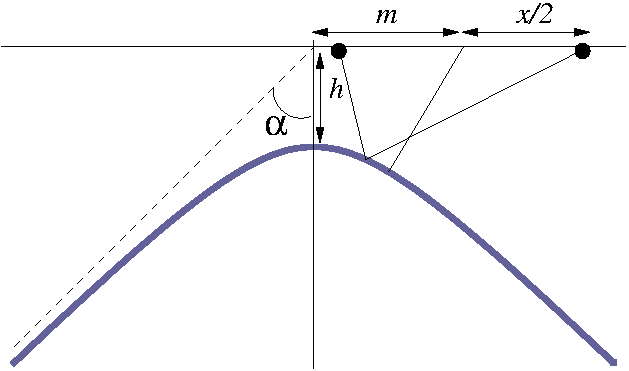
\includegraphics[width=0.11\textwidth]{hyper/Fig/hyper}
    \label{fig:hyper}}
    \subfigure[]{\includegraphics[width=0.11\textwidth]{hyper/Fig/hyper0}
    \label{fig:hyper0}}    
  \subfigure[]{\includegraphics[width=0.11\textwidth]{hyper/Fig/hyper-zero}
    \label{fig:hyper-zero}}\\
    \subfigure[]{\includegraphics[width=0.11\textwidth]{hyper/Fig/hyper-seis}
    \label{fig:hyper-seis}}
  \subfigure[]{\includegraphics[width=0.11\textwidth]{hyper/Fig/hyper-fx}
    \label{fig:hyper-fx}}
  \subfigure[]{\includegraphics[width=0.11\textwidth]{hyper/Fig/hyper-seisvd}
    \label{fig:hyper-seisvd}}
	\caption{(a) Original synthetic data. (b) Under-sampled data. (c) Zero padded data (50\% traces regularly removed). (d) Reconstructed data by using traditional iterative seislet thresholding. (e) Reconstructed data by using Spitz's method. (f) Reconstructed data by using the proposed approach.}
   \label{fig:hyper,hyper0,hyper-zero,hyper-seis,hyper-fx,hyper-seisvd}
\end{figure}

\section{Method}
\subsection{Projection onto convex sets (POCS)}
The principal problem of seismic data reconstruction is to solve the underdetermined inversion problem:
\begin{equation}
\label{eq:acq}
\mathbf{Sm}=\mathbf{d},
\end{equation}
where $\mathbf{m}$ is the well-sampled seismic data (or model), $\mathbf{S}$ denotes the sampling operator, and $\mathbf{d}$ denotes the observed data \cite{yangkang2014halfthr}. Because of the missing traces, the operator $\mathbf{S}$ is highly singular and thus makes equation \ref{eq:acq} highly underdetermined.

There have been many different algorithms for solving equation \ref{eq:acq} by imposing different constraints. In the seismic data processing field, the POCS algorithm \cite{abma2006} is one of the most widely used methods to interpolate seismic data with irregularly missing traces, and has the following iterative expression:
\begin{equation} 
\label{eq:pocs}
\mathbf{m}_{n+1}=\mathbf{d}+(\mathbf{I}-\mathbf{S})\mathbf{A}^{-1}\mathbf{T}\mathbf{A}[\mathbf{m}_n],
\end{equation}
where $\mathbf{m}_n$ denotes the reconstructed data after $n$th iteration, $\mathbf{A}$ and $\mathbf{A}^{-1}$ are the forward and inverse sparsity-promoting transforms, $\mathbf{I}$ is an identity matrix and $\mathbf{T}$ is a thresholding operator. However, for regularly missing traces, POCS can not obtain satisfied results because of the strong aliasing noise in the sparse domain. \cite{shuwei20153} has shown that the seislet-based POCS algorithm can still be effective for interpolating regularly missing traces provided that an accurate local slope map can be obtained. All the examples in this paper are based on the iterative framework \ref{eq:pocs}. The thresholding operator $\mathbf{T}$ is chosen as a soft-thresholding operator in the seislet domain:
\begin{equation}
\label{eq:soft}
%\mathbf{\mathcal{T}}_{\gamma_i} (\mathbf{x}) =
\mathbf{T}_{\gamma}(v(\mathbf{x})) = \left\{ \begin{array}{ll}
v(\mathbf{x})-\gamma \frac{v(\mathbf{x})}{|v(\mathbf{x})|} & \text{for}\quad  |v(\mathbf{x})| > \gamma  \\
0			      & \text{for}\quad  |v(\mathbf{x})| \le \gamma
\end{array}\right.,
\end{equation}
where $\mathbf{T}_{\gamma}$ corresponds to the soft thresholding operator with a threshold value $\gamma$.  $\mathbf{x}$ denotes the coordinates vector. $v(\mathbf{x})$ denotes the value the spatial point $\mathbf{x}$.

\subsection{Dealiased interpolation by low-frequency constrained iterative local slope estimation}
 When interpolating the regularly missing traces by using a seislet-based POCS algorithm, there are three key factors that can affect the final reconstruction results: (1) The slope estimation. (2) The threshold value in the seislet transform. (3) The number of iterations. For the traditional approach, we calculate the local slope every a small number of iterations using the low-frequency components of seismic data. The large number of iterations is also used to ensure an acceptable slope estimation. The threshold value is designed assuming that a constant percentage of transform coefficients can optimally represent the true data. In the next section, we propose a very effective and efficient way for improving the traditional interpolation by using a different slope estimation approach, which is efficient and accurate enough to allow us to obtain a successful interpolation performance through a fairly small number of iterations. 

\subsection{Dealiased interpolation via one-step local slope estimation based on velocity-slope transformation}
The estimation of the local slope in highly under-sampled data is a challenging problem. Instead of estimating the local slope by using the plane-wave destruction (PWD) algorithm \cite{fomel2002pwd} directly, we first calculate the NMO velocity  by using simple NMO-correction based velocity analysis and then transform the NMO velocity to local slope \cite{liuyang2013} by using
\begin{equation}
\label{eq:vtop}
p(t,x)=\frac{x}{t(x)v_n^2(t_0,x)},
\end{equation}
where $t_0$ is the zero-offset traveltime, $t(x)$ is the traveltime recorded at offset $x$, $v_n(t_0,x)$ is the NMO velocity, and $p(t,x)=dt/dx$ is the local slope. It is salient that $p(t,x)>0$ when $x>0$, as shown by the example in Fig. \ref{fig:hyper,hyper0,hyper-zero,hyper-seis,hyper-fx,hyper-seisvd}. The detailed velocity-slope transformation was introduced in \cite{liuyang2013}. It should be mentioned that such velocity-slope transformation was used previously by \cite{liuyang2015} and \cite{shuwei2016} for signal and noise separation. We use the velocity-slope transformation here for iterative interpolation based on seislet thresholding. We admit here that since equation \ref{eq:vtop} is derived from prestack data, the iterative interpolation approach based on the velocity-slope transformation cannot be applied to poststack seismic data processing, where the data structure can be arbitrarily complex and local slope can vary rapidly. Although prestack data can also be complex, we limit our algorithm in a simpler case, where we assume that the prestack data structure is relatively simple and do not have negative slope. As far as we know, this assumption is satisfied in most situations. 

The seislet transform has found successful applications in noise attenuation \cite{seislet,yangkang20142}. However, the successful application of the seislet transform in iterative interpolation, especially in the industry, is not reported often. One of the drawbacks that impede the wide application of seislet based interpolation is the efficiency. The seislet transform itself does not slow down the efficiency too much. However, the slope estimation that is required by the seislet transform is much slower. The efficiency of seislet transform is about 2-4 times slower than the fast Fourier transform, and is about 4-8 times slower than the fast wavelet transform \cite{seislet}.   In order to accelerate the process, the slope estimation is commonly estimated every several iterations.  

In \cite{shuwei20153}, the slope estimation is iterated every 5 iterations. Even though, the computational cost is still much heavier than the widely used Fourier transform. In this letter, the one-step slope estimation from velocity-slope transformation (shown in equation \ref{eq:vtop}) can greatly improve the efficiency by reducing numerous cost in iterative slope estimation. According to the performance of the synthetic example in the letter, the more accurate slope can even make the finally reconstructed data more accurate.  Thus, the utilization of velocity-slope transformation in seislet-based interpolation could be of a huge influence on promoting the wide application of seislet based interpolation approach in the industry. 

\section{Examples}
We present two examples to show the superior performance  by using the proposed algorithm and the significance of one-step slope estimation.  The first example is shown in Fig. \ref{fig:hyper,hyper0,hyper-zero,hyper-seis,hyper-fx,hyper-seisvd}. Fig. \ref{fig:hyper} shows the original data. Fig. \ref{fig:hyper0} shows the under-sampled data by removing 50\% traces. Fig. \ref{fig:hyper-zero} shows the zero-padded section. It is worth mentioning that in the interpolation based inverse problem, Fig. \ref{fig:hyper-zero} is treated as the observed data with preprocessing done on Fig. \ref{fig:hyper0} (adding the zero traces). Fig. \ref{fig:hyper} is treated as the true model. The reconstruction results are compared with Fig. \ref{fig:hyper} to evaluate the performance.  Figs. \ref{fig:hyper-seis}, \ref{fig:hyper-fx}, and \ref{fig:hyper-seisvd} show the interpolated results by using traditional iterative seislet thresholding approach, prediction based approach, and the proposed approach, respectively. All the three methods seem to obtain good results.   Fig. \ref{fig:hyper-seis-dif,hyper-fx-dif,hyper-seisvd-dif} shows the reconstruction error by using three different approaches. There is nearly no error in most portion of the profile except for some small ones between 1s and 1.5s for the proposed approach (Fig. 2(c)). However, the other two approaches will cause significantly more useful energy damages. Fig. \ref{fig:hyper-sdip,hyper-pdip,hyper-dipiter,hyper-vdip} shows the calculated slope for different datasets. The slope estimated by using the velocity-slope transformation is almost the same as the true slope, while the slope via iterative low-frequency constrained estimation has a much larger error.  In order to numerically compare the reconstruction performance, the signal-to-noise ratio (SNR) is also used here, which was defined as \cite{herrmann,yangkang2015ortho}:
\begin{equation}
\label{eq:snr}
SNR_n=10\log_{10}\frac{\Arrowvert \mathbf{m}_{true} \Arrowvert_2^2}{\Arrowvert \mathbf{m}_{true} -\mathbf{m}_n\Arrowvert_2^2}.
\end{equation}
where $\mathbf{m}_n$ denotes the reconstructed data after $n$th iteration, and $\mathbf{m}_{true}$ denotes the true model.
The SNRs comparison between the traditional seislet thresholding and the proposed seislet thresholding are shown in Figs. \ref{fig:snrs-pocs} and \ref{fig:snrs-pocsvd}. It is obvious that in addition to the tremendous computational cost reduced by the one-step estimation and less desired number of iterations, the proposed approach can also improve the final reconstructed result. The converged SNR by using the proposed approach after 40 iterations is about 27 dB, while the SNR by using the traditional approach after  200 iterations is only about 15 dB. Besides, from the SNR diagrams, we can also infer that the traditional approach might not be stable after a large number of iterations because of the error accumulation on the slope, since the SNR starts to decrease after about 150 iterations.


In order to test the influence of noise, we add some background noise to the synthetic example and conduct the same experiment as the clean data example. Figs. \ref{fig:hyper-n,hyper0-n,hyper-zero-n,hypern-seis,hypern-fx,hypern-seisvd} and \ref{fig:hypern-seis-dif,hypern-fx-dif,hypern-seisvd-dif} show the reconstruction performance for the noisy data.  Figs. \ref{fig:hyper-n}, \ref{fig:hyper0-n}, and \ref{fig:hyper-zero-n} show the noisy counterparts of Figs.  \ref{fig:hyper}, \ref{fig:hyper0}, and \ref{fig:hyper-zero}. Figs. \ref{fig:hypern-seis}, \ref{fig:hypern-fx}, and \ref{fig:hypern-seisvd} show the reconstructed results by using three different methods. Figs. \ref{fig:hypern-seis-dif}, \ref{fig:hypern-fx-dif}, and \ref{fig:hypern-seisvd-dif} show their corresponding error sections. In this noisy data experiment, the true model is still the clean data shown in Fig. \ref{fig:hyper}. By comparing the figures in Figs. \ref{fig:hyper-n,hyper0-n,hyper-zero-n,hypern-seis,hypern-fx,hypern-seisvd} and \ref{fig:hypern-seis-dif,hypern-fx-dif,hypern-seisvd-dif}, we can get a similar conclusion as the clean data experiment. The proposed approach can obtain the best performance, although the overall performance is worse than the clean data experiment. In this case, Spitz's method causes a lot of residual noise in the final result, since it is based on the prediction filter, which will inevitably predict the random noise. 

The next example is a poorly sampled marine dataset, which is shown in Fig. \ref{fig:bei}. Fig. \ref{fig:bei-zero} shows the zero-padded data. Fig. \ref{fig:vscan} shows the NMO-based velocity analysis. The black string denotes the automatically picked NMO velocity. Fig. \ref{fig:bei-pdip} shows the local slope calculated directly from the noisy and incomplete data by using the PWD algorithm (Fig. \ref{fig:bei-zero}). Fig. \ref{fig:bei-vdip} shows the obtained local slope by using the velocity-slope transformation equation \ref{eq:vtop}. The slope calculated through PWD algorithm is far from reasonable to capture the true local slope information of the data while the slope from the velocity-slope transformation can be interpreted well. Thus the latter method can be more stable in dealing with highly incomplete and noisy field datasets. Figs. \ref{fig:bei-fx} shows the result by using Spitz's method. Fig. \ref{fig:bei-seisvd} shows the result by using the proposed approach, which is of higher quality than Spitz's method. Figs. \ref{fig:fk-bei,fk-bei-zero,fk-bei-fx,fk-bei-seisvd} shows the corresponding FK spectrum of different datasets, which also confirms that the aliasing problem is no longer existing after implementation of the proposed method.  If observed carefully, some low-frequency low-wavenumber components can be discerned in Fig. \ref{fig:fk-bei-seisvd}. In order to know exactly what these spectrum components represent in the time-space domain, we filter the final reconstructed result with a simple bandpass filter (with a bound frequency 9 Hz) and show the filtered result in Fig. \ref{fig:bei-seis-bp}. Although we can not see obvious differences between Figs. \ref{fig:bei-seisvd} and \ref{fig:bei-seis-bp}, we can find something in their difference section, as shown in Fig. \ref{fig:bei-dif-bp}. The data shown on Fig. \ref{fig:bei-dif-bp} corresponds to the low-frequency and low-wavenumber components of the field data, which is however very important to many seismic data processing tasks such as waveform inversion. Figs. \ref{fig:fk-bei-seis-bp} and \ref{fig:fk-dif-bp} show the FK spectrum of Figs. \ref{fig:bei-seis-bp} and \ref{fig:bei-dif-bp}, respectively. Figs. \ref{fig:fk-bei-seis-bp} and \ref{fig:fk-dif-bp} not only demonstrate the correctness of the bandpass filter, but also confirm the low-frequency data recovery property of the proposed algorithm. 



\section{Conclusion}
The seislet-based POCS algorithm can be used to interpolate regularly missing traces, but requires a fairly accurate local slope estimation. The iterative slope estimation strategy may not always  be successful, which will degrade the final interpolation performance. We propose a more stable way for calculating the local slope by using the velocity-slope transformation, which reduces the number of iterations needed in interpolation and can significantly improve the interpolation performance. Results from both synthetic and field data examples show that the proposed seislet-based POCS algorithm with one-step slope estimation can efficiently and effectively reconstruct the regularly missing traces.

\begin{figure}[htb!]
  \centering
  \subfigure[]{\includegraphics[width=0.11\textwidth]{hyper/Fig/hyper-seis-dif}
    \label{fig:hyper-seis-dif}}
    \subfigure[]{\includegraphics[width=0.11\textwidth]{hyper/Fig/hyper-fx-dif}
    \label{fig:hyper-fx-dif}}
    \subfigure[]{\includegraphics[width=0.11\textwidth]{hyper/Fig/hyper-seisvd-dif}
    \label{fig:hyper-seisvd-dif}}         
	\caption{(a) Reconstruction error by using the traditional iterative seislet thresholding. (b) Reconstruction error by using Spitz's method. (c) Reconstruction error by using the proposed approach.  }
   \label{fig:hyper-seis-dif,hyper-fx-dif,hyper-seisvd-dif}
\end{figure}

\begin{figure}[htb!]
  \centering
    \subfigure[]{\includegraphics[width=0.14\textwidth]{hyper/Fig/snrs-pocs}
    \label{fig:snrs-pocs}}
  \subfigure[]{\includegraphics[width=0.14\textwidth]{hyper/Fig/snrs-pocsvd}
    \label{fig:snrs-pocsvd}}       
	\caption{(a) SNRs by using the traditional iterative seislet thresholding. (b) SNRs by using the proposed approach. Please note that a large number of iterations can be saved and the performance can be improved.}
   \label{fig:snrs-pocs,snrs-pocsvd}
\end{figure}

\begin{figure}[htb!]
  \centering
    \subfigure[]{\includegraphics[width=0.10\textwidth]{hyper/Fig/hyper-sdip}
    \label{fig:hyper-sdip}}
  \subfigure[]{\includegraphics[width=0.10\textwidth]{hyper/Fig/hyper-pdip}
    \label{fig:hyper-pdip}}
    \subfigure[]{\includegraphics[width=0.10\textwidth]{hyper/Fig/hyper-dipiter}
    \label{fig:hyper-dipiter}}
    \subfigure[]{\includegraphics[width=0.10\textwidth]{hyper/Fig/hyper-vdip}
    \label{fig:hyper-vdip}}         
	\caption{(a) True slope. (b) Slope from PWD. (c) Slope estimated iteratively. (d) Slope from velocity-slope transformation.  }
   \label{fig:hyper-sdip,hyper-pdip,hyper-dipiter,hyper-vdip}
\end{figure}


\begin{figure}[htb!]
  \centering
    \subfigure[]{\includegraphics[width=0.11\textwidth]{hypern/Fig/hyper-n}
    \label{fig:hyper-n}}
    \subfigure[]{\includegraphics[width=0.11\textwidth]{hypern/Fig/hyper0-n}
    \label{fig:hyper0-n}}    
  \subfigure[]{\includegraphics[width=0.11\textwidth]{hypern/Fig/hyper-zero-n}
    \label{fig:hyper-zero-n}}\\
    \subfigure[]{\includegraphics[width=0.11\textwidth]{hypern/Fig/hypern-seis}
    \label{fig:hypern-seis}}
  \subfigure[]{\includegraphics[width=0.11\textwidth]{hypern/Fig/hypern-fx}
    \label{fig:hypern-fx}}
  \subfigure[]{\includegraphics[width=0.11\textwidth]{hypern/Fig/hypern-seisvd}
    \label{fig:hypern-seisvd}}
	\caption{(a) Noisy synthetic data. (b) Under-sampled data. (c) Zero padded data (50\% traces regularly removed). (d) Reconstructed data by using traditional iterative seislet thresholding. (e) Reconstructed data by using Spitz's method. (f) Reconstructed data by using the proposed approach.}
   \label{fig:hyper-n,hyper0-n,hyper-zero-n,hypern-seis,hypern-fx,hypern-seisvd}
\end{figure}

\begin{figure}[htb!]
  \centering
  \subfigure[]{\includegraphics[width=0.11\textwidth]{hypern/Fig/hypern-seis-dif}
    \label{fig:hypern-seis-dif}}
    \subfigure[]{\includegraphics[width=0.11\textwidth]{hypern/Fig/hypern-fx-dif}
    \label{fig:hypern-fx-dif}}
    \subfigure[]{\includegraphics[width=0.11\textwidth]{hypern/Fig/hypern-seisvd-dif}
    \label{fig:hypern-seisvd-dif}}         
	\caption{Noisy data example. (a) Reconstruction error by using the traditional iterative seislet thresholding. (b) Reconstruction error by using Spitz's method. (c) Reconstruction error by using the proposed approach.  }
   \label{fig:hypern-seis-dif,hypern-fx-dif,hypern-seisvd-dif}
\end{figure}

\begin{figure*}[ht!]
  \centering
    \subfigure[]{\includegraphics[width=0.125\textwidth]{bei/Fig/bei}
    \label{fig:bei}}   
  \subfigure[]{\includegraphics[width=0.125\textwidth]{bei/Fig/bei-zero}
    \label{fig:bei-zero}}
  \subfigure[]{\includegraphics[width=0.125\textwidth]{bei/Fig/vscan}
    \label{fig:vscan}}  \\
  \subfigure[]{\includegraphics[width=0.115\textwidth]{bei/Fig/bei-pdip}
    \label{fig:bei-pdip}}        
  \subfigure[]{\includegraphics[width=0.115\textwidth]{bei/Fig/bei-vdip}
    \label{fig:bei-vdip}}     
  \subfigure[]{\includegraphics[width=0.115\textwidth]{bei/Fig/bei-fx}
    \label{fig:bei-fx}}
  \subfigure[]{\includegraphics[width=0.115\textwidth]{bei/Fig/bei-seisvd}
    \label{fig:bei-seisvd}}
	\caption{(a) Original under-sampled field data.  (b) Zero padded data (with 50\% traces regularly removed). (c) Velocity analysis result. (d) Local slope calculated directly from (b) by using the PWD algorithm. (e) Local slope calculated from the velocity-slope transformation. (f) Reconstructed data by using Spitz's method. (g) Reconstructed data by using the proposed approach.  }
   \label{fig:bei,bei-zero,vscan,bei-vdip,bei-fx,bei-seisvd}
\end{figure*}


\begin{figure*}[ht!]
  \centering
    \subfigure[]{\includegraphics[width=0.115\textwidth]{bei/Fig/fk-bei}
    \label{fig:fk-bei}}   
  \subfigure[]{\includegraphics[width=0.115\textwidth]{bei/Fig/fk-bei-zero}
    \label{fig:fk-bei-zero}}
  \subfigure[]{\includegraphics[width=0.115\textwidth]{bei/Fig/fk-bei-fx}
    \label{fig:fk-bei-fx}}
  \subfigure[]{\includegraphics[width=0.115\textwidth]{bei/Fig/fk-bei-seisvd}
    \label{fig:fk-bei-seisvd}}
	\caption{FK spectrum of different sections. (a) Original under-sampled field data. (b) Zero padded data (with 50\% traces regularly removed). (c) Reconstructed data by using Spitz's method. (d) Reconstructed data by using the proposed approach.  }
   \label{fig:fk-bei,fk-bei-zero,fk-bei-fx,fk-bei-seisvd}
\end{figure*}


\begin{figure}[htb!]
  \centering
    \subfigure[]{\includegraphics[width=0.12\textwidth]{bei/Fig/bei-seis-bp}
    \label{fig:bei-seis-bp}}
  \subfigure[]{\includegraphics[width=0.12\textwidth]{bei/Fig/bei-dif-bp}
    \label{fig:bei-dif-bp}}\\
    \subfigure[]{\includegraphics[width=0.12\textwidth]{bei/Fig/fk-bei-seis-bp}
    \label{fig:fk-bei-seis-bp}}       
    \subfigure[]{\includegraphics[width=0.12\textwidth]{bei/Fig/fk-dif-bp}
    \label{fig:fk-dif-bp}}       
	\caption{(a) Bandpass filtered result after iterative seislet thresholding with a bound frequency 9 Hz. (b) Low frequency data of the reconstructed data in Fig. \ref{fig:bei-seisvd}. (c) FK spectrum of (a). (d) FK spectrum of (b).  }
   \label{fig:bei-seis-bp,bei-dif-bp,fk-bei-seis-bp,fk-dif-bp}
\end{figure}

\section{Acknowledgments}
This research is partially supported by National Science and Technology Major Project of China under Grants No. 2011ZX05024-001-01 and Texas Consortium for Computational Seismology (TCCS). %Moreover, we are also grateful for the support of the Australian and Western Australian Governments and the North West Shelf Joint Venture Partners, as well as the Western Australian Energy Research Alliance. 

\bibliographystyle{IEEEtran}
\bibliography{dealiase}







